\section{Where the two processors spend their time}
\label{sec:parallel:limits}

\Cref{sec:parallel:why} of the paper explains the device's disadvantage in
structural terms; the hardware counters below identify the resource each
processor is short of.
\Cref{tab:counters} is Nsight Compute over the device search kernel and
\cref{tab:counters-host,tab:symbols} are \texttt{perf} on the host, six scenes
each, at the \op{Tight} mode and the shipped parameters.

\paragraph{Memory traffic.} The device is not short of bandwidth. Across the
six scenes the search moves between $0.8$ and $220\,\mathrm{MB}$ of dynamic
random-access memory (DRAM) traffic per launch, and never exceeds $1.2\%$ of
sustained DRAM peak. Arithmetic needs more care, because the natural measure of
it is the wrong one here. \Cref{tab:pipes} reports what the units are doing, and
\cref{tab:throughput} reports the throughput that matters here, candidate pairs
resolved per second. The cache hierarchy explains the quiet memory system. On
armadillo-rollers the kernel touches $63.9\,\mathrm{MB}$ of L1 sectors,
$20.3\,\mathrm{MB}$ of those reach L2, and only $2.3\,\mathrm{MB}$ reach DRAM. A
box is small, and its parent's corners are still resident when its children are
built.

\paragraph{Functional-unit utilisation.} The functional units are not idle; the
multiprocessor is. Two columns of \cref{tab:pipes} are normalised differently.
The pipe columns give each unit's share of its peak issue rate \emph{while the
multiprocessor is active}, and on that basis the double-precision pipe runs at
$18$ to $29\%$ of peak and the integer arithmetic logic unit (ALU) at $15$ to
$25\%$, close behind it on every scene. The \emph{SM} column is the whole
multiprocessor's share of peak over \emph{elapsed} time, and on the smallest
scene it is $2.25\%$. Pipes that issue at a quarter of peak when they have warps
to issue from do not limit this kernel, and cheaper arithmetic would not move
it.

The elapsed-time column also shows where the grid stops mattering. It climbs with
the launch size, from $2.25\%$ at $0.41$ waves per multiprocessor to $28.4\%$ at
$4.44$, and then stops: n-body and puffer-ball, at $333$ and $475$ waves, reach
$26.4\%$ and $28.6\%$. Four waves is enough to cover the device, and the hundred
after that buy nothing.

No flop rate is reported here. A rate against arithmetic peak is the figure of
merit for a dense kernel, whose work is fixed and whose only question is how
fast it can be pushed through, whereas the work of a branch-and-bound search is
not fixed and the whole design exists to do less of it. Corner inheritance in
\cref{alg:host} turns eight corner evaluations into four, and sharing a bound
across queries takes the search from about eleven boxes per query to roughly
one. Both cut the flop count, and both make the implementation better. An
implementation that raised its flop rate while returning the same answers would
be a worse one. The rate therefore carries no information about quality, and the
comparison against peak none about headroom. What we claim from the pipe columns
is narrower: no functional unit is saturated, so no functional unit is the
limit.

The instruction mix settles one more question, the kind of arithmetic the search
does. Integer thread-instructions run at $0.58$ to $0.95$ per double-precision
instruction, so the kernel does nearly as much integer work as floating-point
work. That integer work is the algorithm itself: stack indices, query
identifiers, depth counters, the barycentric validity test and the atomics of
\cref{alg:device}. A corner evaluation is double-precision work, and a box is
more than a corner evaluation. The load-store pipe never exceeds $8.1\%$, the
instruction-side counterpart of the quiet DRAM above.

\begin{figure}[htbp]
  \centering
  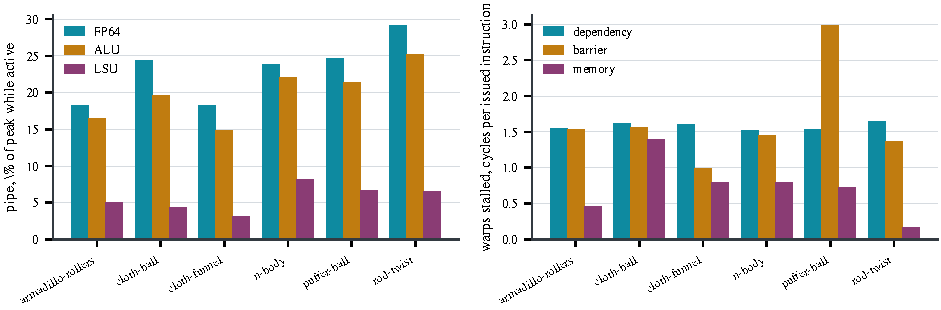
\includegraphics[width=\linewidth]{figures/device-counters.pdf}
  \caption{Device counters per scene. Left: each pipe's share of its peak issue
    rate while the multiprocessor is active. Right: warps stalled per issued
    instruction, by reason. The dependency term is flat across inputs whose
    launches differ by three orders of magnitude, which is the observation
    \cref{sec:parallel:limits} rests on. The tables are
    \cref{tab:pipes,tab:counters}.}
  \label{fig:counters}
\end{figure}

\paragraph{Available parallelism.} The kernel is not short of work to schedule
either, and six scenes establish this where two would not. The grid size spans
three orders of magnitude, from $0.41$ waves per multiprocessor on cloth-funnel,
where the launch does not cover the device even once, to $475$ on puffer-ball,
where it covers it hundreds of times over. Occupancy moves hardly at all across
that range, from $8.4\%$ to $16.3\%$, and the issue rate stays between $0.20$
and $0.35$ instructions per scheduler cycle out of a possible one. A kernel
short of parallelism would improve when handed four hundred times as much of it,
and this one does not.

\paragraph{Latency.} The limit is latency, and the same latency on every scene.
The last three columns of \cref{tab:counters} report the stall terms. Warps
stalled on an execution dependency sit between $1.52$ and $1.65$ on every scene,
a spread of $8\%$ across inputs whose launches differ by three orders of
magnitude in size and whose candidate pairs per step differ by a factor of seven
hundred. Stalls on memory are the smallest term almost everywhere, between
$0.17$ and $1.40$. A corner evaluation is a chain of dependent multiply--adds,
and with $8$ to $16\%$ of the warp slots filled, and $8$ to $24$ of a warp's
$32$ lanes doing useful work when an instruction issues, there are not enough
independent warps resident to cover that chain. Adding grid does not add
residency.

Barrier stalls are the one term that does move, from $0.99$ to $2.98$, with
puffer-ball at the top of that range. Three block-wide barriers per iteration
cost what the slowest thread in the block costs, and puffer-ball has both the
most candidate pairs per step and the widest spread of query difficulty. The
stall does not decide the outcome: puffer-ball's device narrow phase leads the
host by $16.51\times$ in \cref{tab:processor}, the largest such margin in the
benchmark. The counter bounds how much of that margin the barriers cost, and not
whether the device wins.

\paragraph{Host counters.} Grace is the opposite case. The host pipeline retires
between $2.8$ and $3.8$ instructions per cycle at an L1 data miss rate of $0.2$
to $2.1\%$, and the narrow phase on its own misses L1 on between $0.01$ and
$0.65\%$ of loads. The per-lane geometry replication of \cref{sec:parallel:host}
turns a gather into contiguous loads, and the counters show it doing so: a
lane's working set stays resident. Its instruction rate tracks how hard the
queries are and not how many there are. It is $0.49$ on cloth-ball, whose
searches are deep, against $2.87$ on n-body, where the median answer is within
$10^{-8}$ of the root and most queries are settled by a single box. That is the
same dependent chain the device stalls on, paid on a core with enough
out-of-order capacity to hide most of it.

\paragraph{Host costs outside the timings.} \Cref{tab:symbols} attributes
sampled host cycles to the object that spent them. On cloth-funnel $14.1\%$ of
them are inside \texttt{libm}, and the symbol profile puts all of that in one
call, the \texttt{pow} that raises $\delta$ to the third power in
\cref{eq:err}. The share is scene-dependent, falling to $2.6\%$ on
armadillo-rollers. It is written as \texttt{std::pow} deliberately.
\Cref{sec:prelim:err} records that the error bound is certified for one sequence
of operations, and the host keeps the reference's sequence so that its answers
stay bit-identical to it (\cref{sec:results:ref}). The device kernel does not
pay this cost, since it computes $\delta^{3}$ as a plain cube scaled to round
upward. The host could do the same, at the price of the exact agreement that
\cref{sec:results:ref} reports.

The OpenMP runtime is the second such cost, and at its worst it is the largest
of the three: $26.9\%$ of cycles on armadillo-rollers against $0.3\%$ on
puffer-ball. The ordering follows case count and not problem size.
Armadillo-rollers runs $781$ cases and puffer-ball $240$, and each case enters
and leaves the parallel regions of \cref{alg:cell,alg:cellmin} and the narrow
phase afresh. A scene made of many small steps therefore pays the runtime
repeatedly, whereas a scene made of few large ones amortises it away. SCCD's own
code accounts for the rest, between $45$ and $90\%$ of sampled cycles, depending
on how much of the profile the runtime and the operating system take.

\paragraph{Scope of the counters.} These counters cover one narrow-phase mode
and the earliest-impact kernel. The device figures are taken under a profiler
that serialises launches, so they support statements about ratios and none about
absolute time. The host rows are whole-process counters and not per-phase ones.
The pipeline row comes from a build with the device path compiled out, so it is
host work throughout; the narrow-phase row comes from the oracle, which also
drives the device modes, so its instruction rate is a floor. One prediction is
left untested, and it belongs to \cref{sec:parallel:device}: if idle threads
could claim new queries from a global cursor, the dependency and barrier stalls
should fall together. Nothing here confirms that they would.

\begin{table}[!tb]
  \centering
  \caption{Functional-unit use in the device search kernel. The first three
    columns are each pipe's share of its peak issue rate \emph{while the SM is
    active}; \emph{SM} is the whole multiprocessor's share of peak over
    \emph{elapsed} time, so the gap between them is the machine standing idle
    rather than the pipes running slowly. \emph{int/fp64} is integer
    thread-instructions per double-precision one. No flop rate is reported: the
    throughput figure for this pipeline is candidate pairs resolved per second
    (\cref{tab:throughput}), and an implementation that raised its arithmetic
    rate while returning the same answers would be a worse one.}
  \label{tab:pipes}
  \begin{tabular}{lrrrrr}
    \toprule
    & \multicolumn{3}{c}{pipe, \% of peak while active}
      & \multicolumn{2}{c}{} \\
    \cmidrule(lr){2-4}
    scene & FP64 & ALU & LSU & SM \% & int/fp64 \\
    \midrule
    armadillo-rollers & 18.3 & 16.5 & 5.0 & 4.89 & 0.77 \\
    cloth-ball & 24.3 & 19.6 & 4.4 & 4.03 & 0.71 \\
    cloth-funnel & 18.3 & 14.8 & 3.1 & 2.25 & 0.58 \\
    n-body & 23.8 & 22.0 & 8.1 & 26.37 & 0.95 \\
    puffer-ball & 24.6 & 21.4 & 6.7 & 28.61 & 0.90 \\
    rod-twist & 29.1 & 25.2 & 6.6 & 28.43 & 0.72 \\
    \bottomrule
  \end{tabular}
  \par\smallskip\footnotesize Source: \texttt{benchmark/results/profile/}
\end{table}


\begin{table}[!tb]
  \centering
  \caption{Nsight Compute counters for the device narrow-phase kernel, \op{Tight}
    mode, at the shipped parameters. \emph{DRAM} is read and write together for
    one launch and the share of sustained peak bandwidth it represents;
    \emph{lanes} is how many of a warp's $32$ are doing useful work when an
    instruction issues; \emph{issue} is instructions per scheduler cycle out of a
    possible one; \emph{waves} is how many times the grid covers the device. The
    last three columns are warps stalled per issue-active cycle, by reason. A
    profiler serialises launches, so the ratios here are comparable with
    \cref{sec:results} and the absolute times are not.}
  \label{tab:counters}
  \fittable{%
\begin{tabular}{lrrrrrrrrr}
    \toprule
    & \multicolumn{2}{c}{DRAM} & \multicolumn{4}{c}{utilisation}
      & \multicolumn{3}{c}{warps stalled on} \\
    \cmidrule(lr){2-3}\cmidrule(lr){4-7}\cmidrule(lr){8-10}
    scene & MB & \% peak & occ.\ \% & lanes & issue & waves
          & depend. & barrier & memory \\
    \midrule
    armadillo-rollers & 2.28 & 0.085 & 9.0 & 10.2 & 0.20 & 2.24 & 1.55 & 1.54 & 0.46 \\
    cloth-ball & 3.28 & 0.360 & 14.0 & 10.9 & 0.28 & 1.38 & 1.62 & 1.56 & 1.40 \\
    cloth-funnel & 0.84 & 0.082 & 8.4 & 13.8 & 0.20 & 0.41 & 1.60 & 0.99 & 0.80 \\
    n-body & 139.61 & 1.215 & 16.0 & 24.4 & 0.34 & 332.64 & 1.52 & 1.45 & 0.79 \\
    puffer-ball & 219.68 & 1.102 & 16.3 & 18.3 & 0.30 & 475.46 & 1.54 & 2.98 & 0.73 \\
    rod-twist & 5.34 & 0.180 & 14.0 & 8.0 & 0.35 & 4.44 & 1.65 & 1.37 & 0.17 \\
    \bottomrule
  \end{tabular}}
  \par\smallskip\footnotesize Source: \texttt{benchmark/results/profile/}
\end{table}


\begin{table}[!tb]
  \centering
  \caption{\texttt{perf stat} counters on Grace. \emph{pipeline} is the whole
    host pipeline from a build with the device path compiled out, so it is host
    work throughout; \emph{narrow phase} is the accuracy oracle, which runs the
    narrow phase over the curated query sets and no broad phase at all. Both are
    whole-process counters.}
  \label{tab:counters-host}
  \begin{tabular}{lrrrr}
    \toprule
    & \multicolumn{2}{c}{pipeline} & \multicolumn{2}{c}{narrow phase} \\
    \cmidrule(lr){2-3}\cmidrule(lr){4-5}
    scene & inst/cycle & L1 miss \% & inst/cycle & L1 miss \% \\
    \midrule
    armadillo-rollers & 3.29 & 0.73 & 0.80 & 0.35 \\
    cloth-ball & 2.78 & 1.38 & 0.49 & 0.46 \\
    cloth-funnel & 3.35 & 1.31 & 0.84 & 0.55 \\
    n-body & 2.86 & 0.76 & 2.87 & 0.01 \\
    puffer-ball & 3.77 & 2.11 & 1.13 & 0.31 \\
    rod-twist & 3.13 & 0.23 & 0.87 & 0.65 \\
    \bottomrule
  \end{tabular}
  \par\smallskip\footnotesize Source: \texttt{benchmark/results/profile/}
\end{table}


\begin{table}[!tb]
  \centering
  \caption{Where the host spends its cycles, from a sampling profile of the
    CUDA-free build attributed by shared object. \emph{SCCD} is our own code,
    which inlines into the driver; \emph{OpenMP} is the runtime behind the
    parallel loops; \emph{libm} is almost entirely the call that raises $\delta$
    to the third power in \cref{eq:err}. The profile covers the whole process,
    so mesh loading and allocation are in it as well as the pipeline, which is
    most of what the last column holds.}
  \label{tab:symbols}
  \begin{tabular}{lrrrrr}
    \toprule
    scene & SCCD & OpenMP & libm & libc & kernel, other \\
    \midrule
    armadillo-rollers & 48.3 & 26.9 & 2.6 & 16.1 & 6.0 \\
    cloth-ball & 79.9 & 2.0 & 6.3 & 10.1 & 1.6 \\
    cloth-funnel & 44.9 & 6.6 & 14.1 & 3.6 & 30.8 \\
    n-body & 78.3 & 1.5 & 10.7 & 8.4 & 0.9 \\
    puffer-ball & 90.2 & 0.3 & 3.5 & 5.5 & 0.3 \\
    rod-twist & 66.4 & 4.9 & 2.1 & 2.4 & 24.1 \\
    \bottomrule
  \end{tabular}
  \par\smallskip\footnotesize Percentages of sampled cycles.
  Source: \texttt{benchmark/results/profile/}
\end{table}

